\documentclass[crop=false,a4paper,oneside,11pt]{standalone}
\usepackage{a4wide,graphicx,fancyhdr,amsmath,amssymb,float,graphicx,color,geometry,xcolor,titlesec,colortbl,tabu}
\usepackage[parfill]{parskip}
\usepackage[nodayofweek]{datetime}
%----------------------- Macros and Definitions --------------------------

%fast change of things
\newcommand{\mysubject}{2IO70 DBL Embedded Systems}
\newcommand{\myassignment}{Group 12}

%\definecolor{titlepagecolor}{cmyk}{1,.60,0,.40}
%\definecolor{namecolor}{cmyk}{1,.50,0,.10}


\setlength\headheight{20pt}
\addtolength\topmargin{-10pt}
\addtolength\footskip{20pt}

% Define light and dark Microsoft blue colours
\definecolor{MSBlue}{rgb}{.204,.353,.541}
\definecolor{MSLightBlue}{rgb}{.31,.506,.741}
\arrayrulecolor{MSLightBlue}

% Set formats for each heading level

\titleformat*{\section}{\Large\bfseries\sffamily\color{MSBlue}}
\titleformat*{\subsection}{\large\bfseries\sffamily\color{MSLightBlue}}

%date format
\newdateformat{mydate}{\monthname[\THEMONTH] \THEYEAR}

\fancypagestyle{plain}{%
\fancyhf{}
\renewcommand{\headrulewidth}{0pt}
\renewcommand{\footrulewidth}{0pt}
}

\pagestyle{fancy}
\fancyhf{}
\fancyfoot[CO] {\thepage}
\renewcommand{\headrulewidth}{0pt}
\renewcommand{\footrulewidth}{0pt}


%--------------------------------- Text ----------------------------------
\setcounter{secnumdepth}{0}
\begin{document}

\section{Experimental Evaluation}

We ran all the tests in our experimental evaluation on a HP EliteBook 8570w with an Intel i7-3630QM CPU @ 2.40GHz and 8,00 GB RAM. To measure the amount of time and algorithm we start a timer in the code just before the part we want to test and we stop the timer right after the part stops.

\subsection{2-position}
\subsubsection{Results}
The running time of the 2-position algorithm can be seen in figure ...


The percentage of labels placed by the 2-position algorithm can be seen in figure ...
\subsubsection{Discussion}

\subsection{4-position}
\subsubsection{Results}
The running time of the 4-position algorithm can be seen in figure ...
 \begin{figure}[h!]
 \centering
 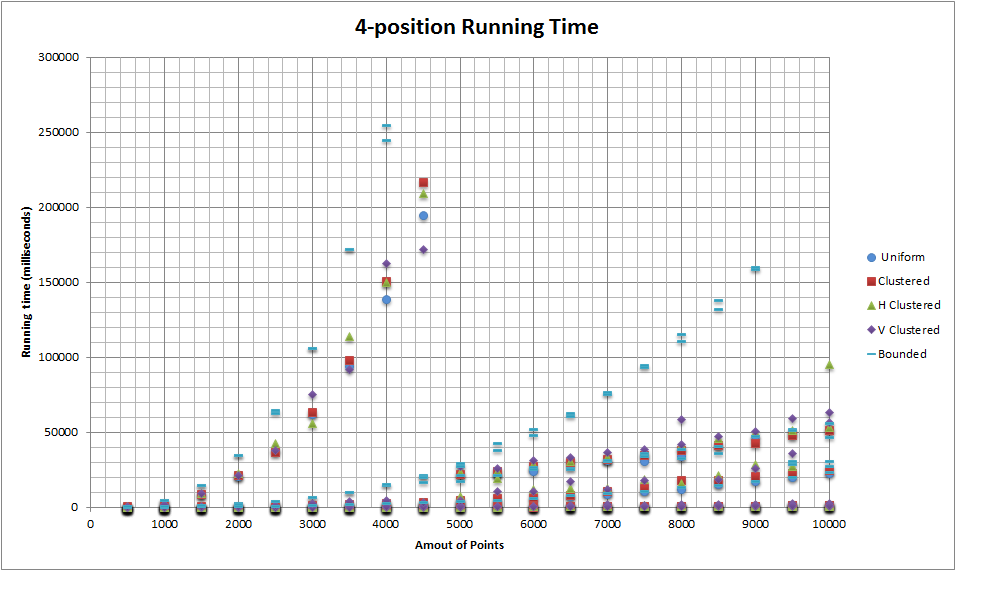
\includegraphics[scale = 0.5]{4PosRunningTime.png}\\
 \caption{A graphic showing the Running Time of the 4-position algorithm}
 \end{figure}

The percentage of labels placed by the 4-position algorithm can be seen in figure ...
 \begin{figure}[h!]
 \centering
  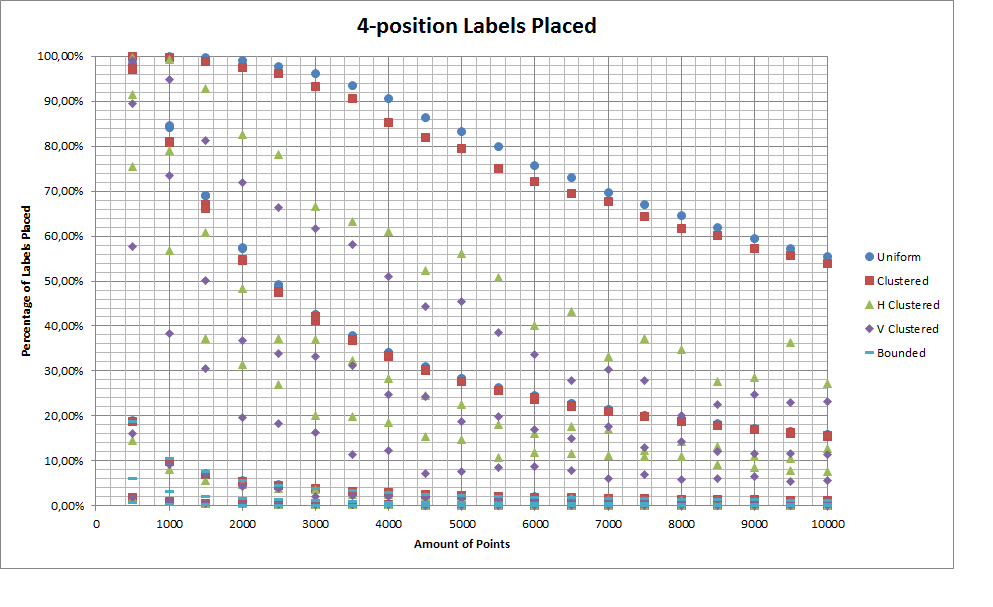
\includegraphics[scale = 0.5]{4PosLabelsPlaced.png}\\
  \caption{A graphic showing the percentage of labels placed by the 4-position algorithm}
 \end{figure}
\subsubsection{Discussion}

\subsection{1-slider}
\subsubsection{Results}
The running time of the 1-slider algorithm can be seen in figure ... We found in practice that the running time of the 1-slider algorithm can exceed the time limit we had of 5 minutes when the amount of overlaps was large. We thus put a hard limit of 4.5 minutes on the heuristic algorithm and, if the algorithm had not given a result by then, ran a greedy algorithm.

The percentage of labels placed by the 1-slider algorithm can be seen in figure ...
\subsubsection{Discussion}

\end{document}
